% ============================================================
%  RAPPORT FINAL — Prédiction d'inactivité de dépôts GitHub
%  ENSA Tétouan | Machine Learning | 2025-2026
% ============================================================
\documentclass[12pt,a4paper]{article}

% ---- Encodage & langue ----
\usepackage[utf8]{inputenc}
\usepackage[T1]{fontenc}
\usepackage[french]{babel}
\usepackage{lmodern}

% ---- Mise en page ----
\usepackage[top=2.5cm, bottom=2.5cm, left=2.8cm, right=2.8cm]{geometry}
\usepackage{setspace}
\onehalfspacing

% ---- Mathématiques ----
\usepackage{amsmath, amssymb}

% ---- Graphiques & couleurs ----
\usepackage{graphicx}
\usepackage{xcolor}
\usepackage{float}
\usepackage{subcaption}

% ---- Tableaux ----
\usepackage{booktabs}
\usepackage{tabularx}
\usepackage{multirow}
\usepackage{longtable}
\usepackage{array}
\usepackage{colortbl}
% Colonnes personnalisees : L = X ragged-right, P{w} = p{w} ragged-right
\newcolumntype{L}{>{\raggedright\arraybackslash}X}
\newcolumntype{P}[1]{>{\raggedright\arraybackslash}p{#1}}

% ---- Code source ----
\usepackage{listings}
\lstset{
  basicstyle=\ttfamily\small,
  keywordstyle=\color{blue}\bfseries,
  commentstyle=\color{gray}\itshape,
  stringstyle=\color{teal},
  numberstyle=\tiny\color{gray},
  numbers=left,
  numbersep=5pt,
  frame=single,
  breaklines=true,
  breakatwhitespace=true,
  showstringspaces=false,
  captionpos=b,
  backgroundcolor=\color{gray!5},
  rulecolor=\color{gray!40},
  xleftmargin=10pt,
  xrightmargin=5pt
}
\lstdefinestyle{python}{language=Python}

% ---- En-têtes & pieds de page ----
\usepackage{fancyhdr}
\pagestyle{fancy}
\fancyhf{}
\fancyhead[L]{\small\textit{Prédiction d'inactivité de dépôts GitHub}}
\fancyhead[R]{\small\textit{ENSA Tétouan --- ML 2025-2026}}
\fancyfoot[C]{\thepage}
\renewcommand{\headrulewidth}{0.4pt}

% ---- Hyperliens ----
\usepackage[hidelinks, colorlinks=true,
            linkcolor=blue!70!black,
            citecolor=green!50!black,
            urlcolor=blue!60!black]{hyperref}

% ---- Autres utilitaires ----
\usepackage{enumitem}
\usepackage{caption}
\usepackage{titlesec}
\usepackage{tcolorbox}
\usepackage{color}
\tcbuselibrary{skins,breakable}

% ---- Couleurs personnalisées ----
\definecolor{ENSAblue}{RGB}{0, 70, 127}
\definecolor{ENSAgray}{RGB}{100, 100, 100}
\definecolor{alertred}{RGB}{200, 0, 0}
\definecolor{successgreen}{RGB}{0, 140, 0}
\definecolor{lightblue}{RGB}{230, 240, 255}
\definecolor{lightyellow}{RGB}{255, 252, 230}

% ---- Boîtes colorées ----
\newtcolorbox{keybox}[1][]{
  colback=lightblue, colframe=ENSAblue,
  fonttitle=\bfseries, title=#1,
  breakable, enhanced
}
\newtcolorbox{warnbox}[1][]{
  colback=lightyellow, colframe=orange!70!black,
  fonttitle=\bfseries, title=#1,
  breakable, enhanced
}

% ---- Style des sections ----
\titleformat{\section}{\Large\bfseries\color{ENSAblue}}{\thesection}{1em}{}[\titlerule]
\titleformat{\subsection}{\large\bfseries\color{ENSAblue!80}}{\thesubsection}{1em}{}
\titleformat{\subsubsection}{\normalsize\bfseries\color{ENSAblue!60}}{\thesubsubsection}{1em}{}

% ============================================================
\begin{document}

% ============================================================
%  PAGE DE GARDE
% ============================================================
\begin{titlepage}
  \newgeometry{top=0cm, bottom=0cm, left=0cm, right=0cm}
  \setlength{\parindent}{0pt}

  % ── Barre bleue supérieure ────────────────────────────────
  \colorbox{ENSAblue}{%
    \parbox{\paperwidth}{%
      \vspace{0.25cm}
      \centering
      \textcolor{white}{\large\bfseries
        École Nationale des Sciences Appliquées de Tétouan}\\[0.1cm]
      \textcolor{white!80!ENSAblue}{\small
        Université Abdelmalek Essaâdi}
      \vspace{0.25cm}
    }%
  }%

  % ── Logo centré sous la barre ─────────────────────────────
  \vspace{0.35cm}
  \begin{center}
    \tcbox[enhanced, arc=6mm, boxrule=0pt,
           colback=white, colframe=white,
           left=2mm, right=2mm, top=2mm, bottom=2mm]{%
      
\includegraphics[height=2.4cm]{ensate_logo.png}%
    }
  \end{center}
  \vspace{0.15cm}

  % ── Corps central ──────────────────────────────────────────
  \begin{center}
    \textcolor{ENSAgray}{\large\bfseries
      Génie Informatique \textbf{---} 2\textsuperscript{ème} Année Cycle Ingénieurs}\\[0.15cm]
    \textcolor{ENSAgray}{\large Module : \textbf{Machine Learning}}

    \vspace{0.5cm}

    % Boîte titre principale
    \begin{tcolorbox}[
      enhanced, arc=5mm, boxrule=1.8pt,
      colframe=ENSAblue, colback=ENSAblue!7,
      drop shadow={ENSAblue!35!black},
      width=0.86\paperwidth,
      left=7mm, right=7mm, top=4mm, bottom=4mm
    ]
      \centering
      {\large\itshape\color{ENSAgray} Rapport Final de Projet}\\[0.25cm]
      {\Huge\bfseries\color{ENSAblue}
        Prédiction d'Inactivité\\[0.15cm]
        de Dépôts GitHub Open Source}\\[0.25cm]
      \textcolor{ENSAblue!50}{\rule{0.55\linewidth}{0.9pt}}\\[0.2cm]
      {\normalsize\itshape\color{ENSAgray}
        Classification supervisée du risque d'abandon\\
        de bibliothèques utilisées comme dépendances logicielles}
    \end{tcolorbox}

    \vspace{1.1cm}

    % Cartes empilées : Réalisé par → Encadrant
    \begin{minipage}[t]{0.50\paperwidth}
      \begin{tcolorbox}[
        enhanced, arc=3mm, boxrule=1pt,
        colframe=ENSAblue, colback=lightblue,
        left=4mm, right=4mm, top=3mm, bottom=3mm
      ]
        \centering
        \textcolor{ENSAblue}{\bfseries\large Réalisé par}\\[0.25cm]
        {\normalsize
          Ismail \textsc{Lyamani}\\[0.12cm]
          Abdellatif \textsc{Oumhella}\\[0.12cm]
          Mohammed Aymane \textsc{Saber}%
        }
      \end{tcolorbox}

      \vspace{0.3cm}

      \begin{tcolorbox}[
        enhanced, arc=3mm, boxrule=1pt,
        colframe=ENSAblue, colback=lightblue,
        left=4mm, right=4mm, top=3mm, bottom=3mm
      ]
        \centering
        \textcolor{ENSAblue}{\bfseries\large Encadrant}\\[0.25cm]
        {\normalsize Pr.~Y.~\textsc{El Younoussi}}
      \end{tcolorbox}
    \end{minipage}

  \end{center}

  \vfill

  % ── Pied de page bleu ──────────────────────────────────────
  \noindent\colorbox{ENSAblue}{%
    \parbox[c][2.0cm]{\paperwidth}{%
      \centering
      \textcolor{white}{\large\bfseries Année universitaire 2025 -- 2026}%
      \quad\textcolor{white!50!ENSAblue}{\large|}%
      \quad\textcolor{white!75!ENSAblue}{\normalsize Date de remise : 3 juin 2026}%
    }%
  }

  \restoregeometry
\end{titlepage}

% ============================================================
%  RÉSUMÉ EXÉCUTIF
% ============================================================
\newpage
\thispagestyle{plain}
\begin{center}
  {\Large\bfseries\color{ENSAblue} Résumé Exécutif}
\end{center}
\vspace{0.3cm}

\begin{keybox}[Abstract]
Ce rapport présente le cycle complet d'un projet de Machine Learning appliqué à la détection proactive de
dépôts GitHub susceptibles d'être abandonnés. La problématique est posée dans un contexte de gestion de
dépendances logicielles : des milliers d'organisations s'appuient sur des bibliothèques \textit{open source}
dont l'abandon peut engendrer des vulnérabilités de sécurité non corrigées.

Un jeu de données original de \textbf{15\,000 dépôts GitHub} a été constitué via l'API REST GitHub
(stratégie d'échantillonnage stratifié en deux passes). Le problème est formulé comme une \textbf{classification
binaire déséquilibrée} (85\,\% actifs / 15\,\% inactifs). Quatre familles de modèles ont été entraînées et
comparées sur trois stratégies de gestion du déséquilibre ; le meilleur modèle (\textbf{Gradient Boosting}
+ \textit{class\_weight}) atteint sur le jeu de test un \textbf{Recall de 0,976}, une \textbf{PR-AUC de 0,900}
et réduit le coût métier estimé de \textbf{663\,360\,\texteuro{} à 96\,920\,\texteuro{}} grâce à
l'optimisation du seuil décisionnel (0,05).

Le modèle est exposé via une \textbf{API REST FastAPI} (déployée sur Railway) et une
\textbf{interface Streamlit} (déployée sur Streamlit Cloud), conteneurisées avec Docker,
permettant des prédictions unitaires et par lot. L'application est accessible publiquement
à l'adresse \url{https://app-repo-activity-classifier.streamlit.app}.
\end{keybox}

\vspace{0.5cm}
\noindent\textbf{Mots-clés :} classification supervisée, déséquilibre de classes, Gradient Boosting,
dépôts GitHub, gestion de dépendances, CRISP-DM, FastAPI, Streamlit, Docker, Railway, Streamlit Cloud.

% ============================================================
%  TABLE DES MATIÈRES
% ============================================================
\newpage
\tableofcontents

% ============================================================
%  LISTE DES FIGURES & TABLEAUX
% ============================================================
\newpage
\listoffigures
\listoftables

\newpage

% ============================================================
%  SECTION 1 — INTRODUCTION ET CONTEXTE MÉTIER
% ============================================================
\section{Introduction et contexte métier}

\subsection{Domaine et problématique}

Dans l'écosystème moderne du développement logiciel, les organisations dépendent massivement de bibliothèques
\textit{open source} hébergées sur des plateformes comme GitHub. Selon le rapport \textit{State of the
Software Supply Chain 2023} de Sonatype~\cite{sonatype2023}, plus de 245\,000 paquets malveillants ou
abandonnés ont été recensés sur les grandes registres (npm, PyPI, Maven Central). Un dépôt abandonné ne
bénéficie plus de correctifs de sécurité, devient incompatible avec les évolutions de son écosystème, et
constitue une dette technique croissante pour ses utilisateurs.

Des incidents réels illustrent l'ampleur des risques : la faille Log4Shell a coûté entre 10\,000\,\texteuro{}
et 500\,000\,\texteuro{} par organisation affectée, et la brèche Equifax (Apache Struts) a abouti à un
règlement de 575 millions de dollars~\cite{snyk2023}.

\begin{warnbox}[Question métier centrale]
\textit{``Peut-on prédire si un dépôt GitHub utilisé comme dépendance ($\geq$ 1 étoile, $\geq$ 30 jours
d'existence) deviendra inactif ou abandonné dans les 6 prochains mois, à partir des métadonnées
disponibles publiquement ?''}
\end{warnbox}

Cette question métier s'inscrit dans la lignée des outils d'analyse de dépendances tels que Snyk,
Dependabot ou Socket.dev, qui cherchent à alerter proactivement les équipes de développement avant que
des risques ne se matérialisent en production.

\subsection{Population cible}

La population cible est définie comme \textbf{l'ensemble des dépôts GitHub publics ayant au moins une
étoile et au moins 30 jours d'existence}. Ce filtre constitue un proxy de visibilité minimale — un
dépôt étoilé a été remarqué par au moins un utilisateur extérieur à l'auteur, ce qui le rend candidat
à être utilisé comme dépendance. Cette définition exclut intentionnellement les projets étudiants,
forks vides et dépôts de tests qui constituent la majorité brute des 420 millions de dépôts GitHub.

\subsection{Objectifs métiers quantifiés}

Le tableau~\ref{tab:objectifs_metier} synthétise les objectifs métiers et leurs critères de succès
définis lors de la phase de cadrage.

\begin{table}[H]
  \centering
  \caption{Objectifs métiers et critères de succès}
  \label{tab:objectifs_metier}
  \begin{tabularx}{\linewidth}{clL}
    \toprule
    \textbf{\#} & \textbf{Objectif métier} & \textbf{Critère de succès} \\
    \midrule
    1 & Identifier au moins 80\,\% des dépôts abandonnés & Recall $\geq 0{,}80$ (classe inactive) \\
    2 & Limiter les fausses alertes & Precision $\geq 0{,}50$ (classe inactive) \\
    3 & Modèle interprétable pour justifier les alertes & Features explicables (pas de boîte noire totale) \\
    \bottomrule
  \end{tabularx}
\end{table}

\subsection{Traduction métier vers ML}

\begin{table}[H]
  \centering
  \caption{Correspondance entre objectifs métiers et objectifs ML}
  \label{tab:traduction_ml}
  \begin{tabularx}{\linewidth}{LLll}
    \toprule
    \textbf{Objectif métier} & \textbf{Objectif ML} & \textbf{Métrique} & \textbf{Seuil} \\
    \midrule
    Détecter 80\,\% des dépôts abandonnés & Maximiser le recall (classe 1) & Recall & $\geq 0{,}80$ \\
    Limiter les faux positifs & Maintenir une précision raisonnable & Precision & $\geq 0{,}50$ \\
    Équilibre recall / précision & Maximiser le F1 & F1-score & $\geq 0{,}65$ \\
    Qualité globale sur données déséquilibrées & Maximiser la PR-AUC & PR-AUC & $\geq 0{,}70$ \\
    \bottomrule
  \end{tabularx}
\end{table}

\subsection{Analyse du coût asymétrique}

L'asymétrie des coûts d'erreur est structurellement déterminante dans ce projet. Le
tableau~\ref{tab:couts} présente une estimation documentée des coûts associés à chaque type d'erreur.

\begin{table}[H]
  \centering
  \caption{Estimation des coûts d'erreur de classification}
  \label{tab:couts}
  \begin{tabularx}{\linewidth}{lL>{\centering\arraybackslash}p{2.8cm}}
    \toprule
    \textbf{Type d'erreur} & \textbf{Scénario et conséquence métier} & \textbf{Coût estimé} \\
    \midrule
    \textbf{Faux Négatif (FN)} &
      \textit{Actif prédit, réellement inactif.}
      L'équipe continue d'utiliser une dépendance vulnérable :
      incident de sécurité, audit d'urgence, downtime. &
      \textcolor{alertred}{\textbf{10\,000\,\texteuro{}}} \\
    \addlinespace
    \textbf{Faux Positif (FP)} &
      \textit{Inactif prédit, réellement actif.}
      Alerte inutile : $\approx$30\,min de vérification par un ingénieur. &
      \textcolor{successgreen}{\textbf{60\,\texteuro{}}} \\
    \bottomrule
  \end{tabularx}
\end{table}

\noindent Le ratio asymétrique est $\approx 167\times$ (FN coûte 167 fois plus qu'un FP). Cette
asymétrie justifie que la \textbf{métrique principale soit le Recall} sur la classe inactive, et que
le seuil de décision soit abaissé sous 0,5.

\subsection{Définition de la variable cible}

\begin{keybox}[Définition opérationnelle de l'inactivité]
Un dépôt est considéré \textbf{inactif (label = 1)} si sa date de dernier \textit{push} est
antérieure de plus de \textbf{180 jours} à la date de collecte :
\[
\texttt{is\_inactive} =
\begin{cases}
  1 & \text{si } \texttt{days\_since\_last\_push} > 180 \\
  0 & \text{sinon}
\end{cases}
\]
Le seuil de 180 jours (6 mois) est suffisamment long pour exclure les dépôts en pause temporaire,
et suffisamment court pour être actionnable dans un cycle de projet standard.
\end{keybox}

\subsection{Métriques retenues}

\begin{table}[H]
  \centering
  \caption{Métriques d'évaluation retenues et refusées}
  \label{tab:metriques}
  \begin{tabularx}{\linewidth}{llL}
    \toprule
    \textbf{Métrique} & \textbf{Statut} & \textbf{Justification} \\
    \midrule
    \textbf{Recall (classe 1)} & \checkmark\ Principale & Minimise les FN --- ratio de coût asymétrique $\approx 167\times$ \\
    F1-score (classe 1) & \checkmark\ Secondaire & Équilibre recall et précision \\
    PR-AUC & \checkmark\ Secondaire & Robuste au déséquilibre, évalue la courbe complète \\
    Precision (classe 1) & \checkmark\ Tertiaire & Contrôle le taux de fausses alertes \\
    Accuracy seule & $\times$\ Refusée & Trompeuse sur données déséquilibrées \\
    ROC-AUC seule & $\times$\ Refusée & Trop optimiste quand la classe négative domine \\
    \bottomrule
  \end{tabularx}
\end{table}

% ============================================================
%  SECTION 2 — DESCRIPTION ET COMPRÉHENSION DES DONNÉES
% ============================================================
\newpage
\section{Description et compréhension des données}

\subsection{Source et collecte}

Le jeu de données a été constitué le \textbf{15 mai 2026} en interrogeant l'\textbf{API REST GitHub
(v2022-11-28)} via le script \texttt{src/data\_collection.py} avec un Personal Access Token en
lecture seule (quota : 5\,000 requêtes/heure).

\begin{table}[H]
  \centering
  \caption{Endpoints GitHub REST utilisés lors de la collecte}
  \label{tab:endpoints_collecte}
  \begin{tabularx}{\linewidth}{lL}
    \toprule
    \textbf{Endpoint} & \textbf{Usage} \\
    \midrule
    \texttt{GET /search/repositories} & Recherche principale --- retourne les métadonnées des dépôts \\
    \texttt{GET /repos/\{owner\}/\{repo\}/contributors} & Nombre de contributeurs distincts \\
    \texttt{GET /repos/\{owner\}/\{repo\}/issues} & 20 dernières issues fermées (délai de réponse) \\
    \texttt{GET /rate\_limit} & Surveillance du quota API \\
    \bottomrule
  \end{tabularx}
\end{table}

\subsubsection{Stratégie d'échantillonnage stratifié en deux passes}

L'API GitHub présente un biais structurel majeur : son tri par défaut (\texttt{updated desc}) renvoie
quasi-exclusivement des dépôts récemment actifs. En pratique, lors des tests initiaux, cette approche
produisait \textbf{0\,\% de dépôts inactifs} dans les résultats. Pour corriger ce biais, une stratégie
en deux passes a été adoptée :

\begin{itemize}[noitemsep]
  \item \textbf{Passe 1} (\texttt{pushed:<cutoff}) : 2\,250 dépôts inactifs garantis (classe minoritaire).
  \item \textbf{Passe 2} (\texttt{pushed:>cutoff}) : 12\,750 dépôts actifs garantis (classe majoritaire).
\end{itemize}

La collecte croise \textbf{7 tranches d'étoiles} × \textbf{10 langages de programmation} (Python,
JavaScript, Java, C++, Go, Ruby, Rust, TypeScript, PHP, C), assurant une diversité représentative en
taille et en activité, et évitant le biais vers les projets très populaires.

\subsection{Description du jeu de données}

\begin{table}[H]
  \centering
  \caption{Caractéristiques générales du jeu de données}
  \label{tab:dataset_dims}
  \begin{tabular}{ll}
    \toprule
    \textbf{Propriété} & \textbf{Valeur} \\
    \midrule
    Nombre de lignes & 15\,000 \\
    Nombre de features & 19 (11 numériques, 2 catégorielles, 6 binaires) \\
    Variable cible & \texttt{is\_inactive} \\
    Classe minoritaire (inactive) & 2\,250 (15{,}0\,\%) \\
    Classe majoritaire (active) & 12\,750 (85{,}0\,\%) \\
    Date de collecte & 15 mai 2026 \\
    \bottomrule
  \end{tabular}
\end{table}

\subsubsection{Validation du ratio de déséquilibre}

Le ratio de 15\,\% d'inactifs n'est ni artificiel ni arbitraire. Avelino et al.~(2019)~\cite{avelino2019}
mesurent $\approx 16\,\%$ de projets GitHub populaires abandonnés sur 1\,932 projets analysés, validant
directement notre cible sur une sous-population qualifiée similaire.

\begin{figure}[H]
  \centering
  \includegraphics[width=0.60\textwidth]{../data/class_distribution.png}
  \caption{Distribution des classes (actif / inactif) dans le jeu de données}
  \label{fig:class_dist}
\end{figure}

\subsection{Schéma des features}

\begin{longtable}{llP{2.5cm}P{5.5cm}}
  \caption{Description des features du jeu de données}\label{tab:features}\\
  \toprule
  \textbf{Feature} & \textbf{Type} & \textbf{Plage/Valeurs} & \textbf{Justification métier} \\
  \midrule
  \endfirsthead
  \multicolumn{4}{c}{\itshape (Suite du tableau~\ref{tab:features})}\\\toprule
  \textbf{Feature} & \textbf{Type} & \textbf{Plage/Valeurs} & \textbf{Justification métier} \\\midrule
  \endhead
  \midrule\multicolumn{4}{r}{\itshape Suite page suivante}\\
  \endfoot
  \bottomrule
  \endlastfoot
  \texttt{stars} & Num. entier & $[0, 500\text{k}+]$ & Popularité et intérêt communautaire \\
  \texttt{forks} & Num. entier & $[0, 100\text{k}+]$ & Utilisation dérivée et engagement actif \\
  \texttt{open\_issues} & Num. entier & $[0, 10\text{k}+]$ & Nombre élevé sans résolution $\Rightarrow$ signal d'abandon \\
  \texttt{watchers} & Num. entier & $[0, 500\text{k}+]$ & Proxy d'intérêt passif soutenu \\
  \texttt{size\_kb} & Num. entier & $[0, 500\text{k}+]$ & Proxy de maturité et de volume de travail \\
  \texttt{repo\_age\_days} & Num. entier & $[30, 5\text{k}+]$ & Dépôts anciens $\Rightarrow$ patterns d'activité distincts \\
  \texttt{contributor\_count} & Num. entier & $[1, 100+]$ & Mono-contributeur $\Rightarrow$ projet structurellement fragile \\
  \texttt{avg\_issue\_response\_hours} & Num. réel & $[-1{,}0, 10\text{k}+]$ & Réponse tardive $\Rightarrow$ maintenance passive \\
  \texttt{engagement\_rate} & Num. dérivé & $[0{,}0, 50{,}0+]$ & $(\text{stars}+\text{forks})/\text{âge}$ --- proxy d'intérêt soutenu \\
  \texttt{stars\_forks\_ratio} & Num. dérivé & $[0{,}1, 1\text{k}+]$ & Distingue projets admirés vs. réellement utilisés \\
  \texttt{language} & Catégorielle & Python, JS, \ldots & Certains langages ont des écosystèmes plus actifs \\
  \texttt{license} & Catégorielle & MIT, Apache, \ldots & Dépôts sans licence souvent abandonnés \\
  \texttt{has\_description} & Binaire & $\{0, 1\}$ & Signal de soin apporté à la documentation \\
  \texttt{has\_homepage} & Binaire & $\{0, 1\}$ & Signal de projet sérieux et maintenu \\
  \texttt{has\_wiki} & Binaire & $\{0, 1\}$ & Signal de documentation active \\
  \texttt{has\_projects} & Binaire & $\{0, 1\}$ & Signal de gestion de projet active \\
  \texttt{is\_fork} & Binaire & $\{0, 1\}$ & Forks $\Rightarrow$ patterns d'activité différents \\
  \texttt{days\_since\_last\_push} & Num.* & $[0, 3\text{k}+]$ & \textcolor{alertred}{Exclu --- data leakage (définit le label)} \\
  \texttt{archived} & Binaire* & $\{0, 1\}$ & \textcolor{alertred}{Exclu --- data leakage (décision post-hoc)} \\
\end{longtable}

\subsection{Analyse exploratoire (EDA)}

\subsubsection{Distribution des langages de programmation}

\begin{figure}[H]
  \centering
  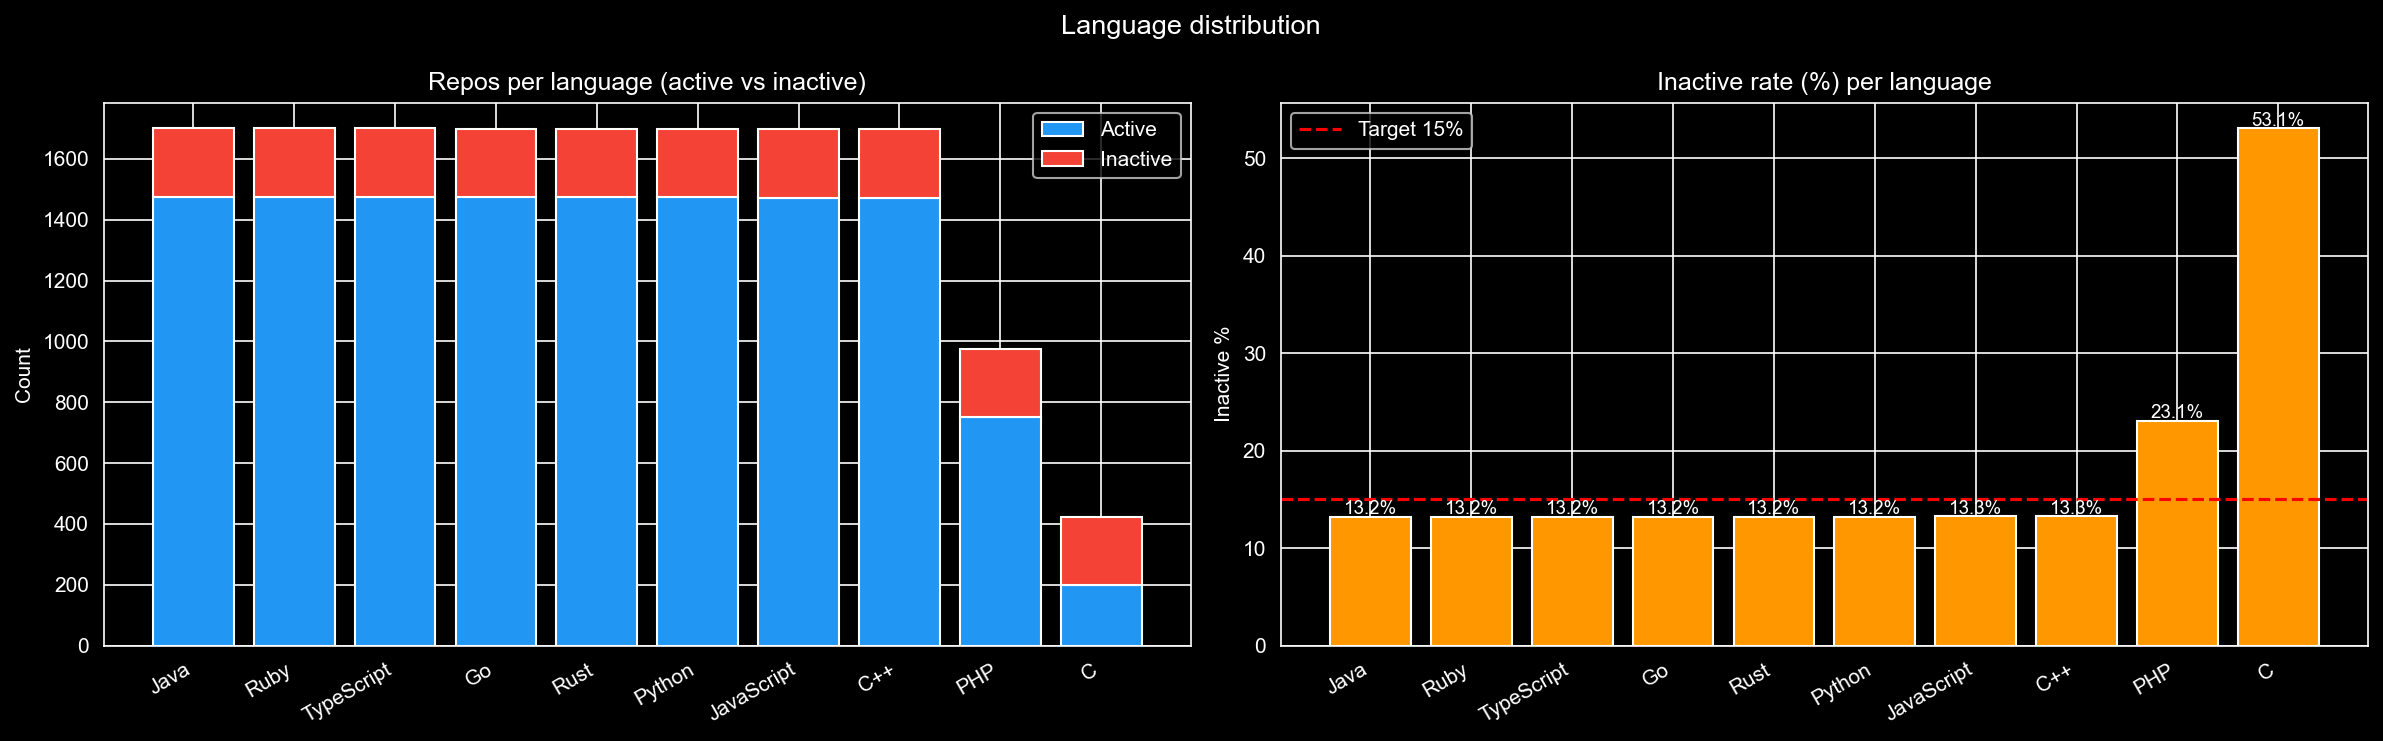
\includegraphics[width=0.75\textwidth]{../data/language_distribution.png}
  \caption{Distribution des langages de programmation dans le jeu de données}
  \label{fig:lang_dist}
\end{figure}

\subsubsection{Matrice de corrélation}

La figure~\ref{fig:corr_matrix} présente la matrice de corrélation entre les variables numériques.
On observe une forte corrélation entre \texttt{stars} et \texttt{watchers} (valeurs souvent
identiques sur GitHub) et une corrélation modérée entre \texttt{engagement\_rate} et \texttt{stars}.

\begin{figure}[H]
  \centering
  \includegraphics[width=0.85\textwidth]{../data/correlation_matrix.png}
  \caption{Matrice de corrélation des variables numériques}
  \label{fig:corr_matrix}
\end{figure}

\subsubsection{Features discriminantes identifiées}

L'analyse bivariée révèle plusieurs features particulièrement discriminantes entre les classes :

\begin{itemize}
  \item \textbf{\texttt{engagement\_rate}} : les dépôts inactifs présentent un taux d'engagement
    nettement plus faible (proche de 0 pour la plupart).
  \item \textbf{\texttt{contributor\_count}} : les dépôts mono-contributeurs sont sur-représentés
    dans la classe inactive.
  \item \textbf{\texttt{repo\_age\_days}} : les dépôts inactifs sont en moyenne significativement
    plus anciens.
  \item \textbf{\texttt{has\_description}} et \textbf{\texttt{has\_homepage}} : corrélés
    positivement avec l'activité.
  \item \textbf{\texttt{avg\_issue\_response\_hours}} : délais plus longs ou valeur sentinelle
    $-1{,}0$ plus fréquente pour les dépôts inactifs.
\end{itemize}

\subsubsection{Limites connues du jeu de données}

\begin{itemize}[noitemsep]
  \item \texttt{contributor\_count} est plafonné à 100 par l'appel à une seule page de l'API.
  \item \texttt{avg\_issue\_response\_hours} vaut $-1{,}0$ pour les dépôts sans issues fermées.
  \item L'API GitHub ne fournit pas la fréquence des commits directement ; \texttt{engagement\_rate}
    en est une approximation.
  \item Les dépôts de moins de 30 jours sont exclus pour éviter de labelliser de nouveaux projets
    comme inactifs.
\end{itemize}

% ============================================================
%  SECTION 3 — PRÉPARATION DES DONNÉES
% ============================================================
\newpage
\section{Préparation des données (Phase 2)}

\subsection{Suppression des variables à risque de data leakage}

Avant toute transformation, quatre colonnes ont été supprimées :

\begin{itemize}[noitemsep]
  \item \texttt{days\_since\_last\_push} --- encode directement le label cible.
  \item \texttt{archived} --- décision post-hoc, souvent consécutive à l'inactivité.
  \item \texttt{full\_name} --- identifiant unique sans valeur prédictive.
  \item \texttt{collected\_at} --- timestamp sans variance utile pour la prédiction.
\end{itemize}

\subsection{Gestion des valeurs manquantes, aberrantes et encodage}

Le tableau~\ref{tab:preprocessing} résume l'ensemble des décisions de preprocessing documentées dans
\texttt{preprocessing\_decisions.md}.

\begin{table}[H]
  \centering
  \caption{Décisions de preprocessing -- récapitulatif}
  \label{tab:preprocessing}
  \small
  \begin{tabularx}{\linewidth}{P{4.2cm}Ll}
    \toprule
    \textbf{Variable} & \textbf{Action appliquée} & \textbf{Scaler/Enc.} \\
    \midrule
    % --- Groupe 1 : Numériques ---
    \rowcolor{ENSAblue!10}
    \multicolumn{3}{l}{\bfseries Variables numériques} \\
    \texttt{avg\_issue\_response\_hours} &
      Valeur $-1{,}0$ $\to$ \texttt{NaN}, imputation par la médiane &
      RobustScaler \\
    \texttt{stars, forks, open\_issues} &
      Conservation des outliers (signaux valides --- loi de puissance) &
      RobustScaler \\
    \texttt{watchers, size\_kb} &
      Conservation &
      RobustScaler \\
    \texttt{repo\_age\_days} &
      Conservation &
      RobustScaler \\
    \texttt{contributor\_count} &
      Conservation (tronqué à 100 par l'API, reste asymétrique) &
      RobustScaler \\
    \texttt{engagement\_rate,}\newline\texttt{stars\_forks\_ratio} &
      Conservation (asymétrie structurelle) &
      RobustScaler \\
    \midrule
    % --- Groupe 2 : Catégorielles ---
    \rowcolor{ENSAblue!10}
    \multicolumn{3}{l}{\bfseries Variables catégorielles} \\
    \texttt{language} &
      Imputation \texttt{most\_frequent}, modalités $<1\,\%$ $\to$ \texttt{'Other'} &
      OneHotEncoder \\
    \texttt{license} &
      Imputation \texttt{most\_frequent}, modalités $<1\,\%$ $\to$ \texttt{'Other'} &
      OneHotEncoder \\
    \midrule
    % --- Groupe 3 : Binaires ---
    \rowcolor{ENSAblue!10}
    \multicolumn{3}{l}{\bfseries Variables binaires} \\
    \texttt{has\_description, has\_homepage,}\newline
    \texttt{has\_wiki, has\_projects, is\_fork} &
      Passthrough (prêts à l'emploi, aucune transformation) &
      --- \\
    \bottomrule
  \end{tabularx}
\end{table}

\begin{keybox}[Justification du RobustScaler]
Le \textbf{RobustScaler} (centrage médiane, mise à l'échelle IQR) a été retenu pour toutes les
features numériques car les distributions de stars, forks et watchers suivent des lois de puissance
avec de nombreuses valeurs extrêmes \textit{réelles}. Ces outliers sont des signaux métier valides
qu'il ne faut pas supprimer, mais dont l'influence sur les modèles sensibles à l'échelle doit être
atténuée.
\end{keybox}

\subsection{Feature Engineering}

Trois nouvelles variables ont été créées pour enrichir la représentation métier :

\begin{enumerate}
  \item \textbf{\texttt{activity\_score}} (indicateur composite d'engagement) :
    \[
      \texttt{activity\_score} = \texttt{stars} + \texttt{forks} + \texttt{watchers}
    \]
    Agrège les trois principaux signaux d'engagement communautaire en un score synthétique.

  \item \textbf{\texttt{issues\_per\_contributor}} (charge de travail par contributeur) :
    \[
      \texttt{issues\_per\_contributor} = \frac{\texttt{open\_issues}}{\texttt{contributor\_count} + 1}
    \]
    Un ratio élevé peut signaler un projet délaissé où peu de contributeurs gèrent un backlog important.

  \item \textbf{\texttt{age\_category}} (discrétisation de l'âge du dépôt) :
    \begin{center}
    \begin{tabular}{ll}
      \toprule
      \textbf{Catégorie} & \textbf{Condition sur \texttt{repo\_age\_days}} \\
      \midrule
      \texttt{nouveau} & $< 180$ jours \\
      \texttt{jeune} & $\in [180, 730)$ jours \\
      \texttt{mature} & $\in [730, 1825)$ jours \\
      \texttt{ancien} & $\geq 1825$ jours \\
      \bottomrule
    \end{tabular}
    \end{center}
    Capture les différentes phases de vie d'un projet ; encodé en One-Hot.
\end{enumerate}

\subsection{Pipeline de preprocessing scikit-learn}

\begin{lstlisting}[style=python, caption={Structure du pipeline de preprocessing (extrait schématique)}, label=lst:pipeline]
from sklearn.pipeline import Pipeline
from sklearn.compose import ColumnTransformer
from sklearn.preprocessing import RobustScaler, OneHotEncoder
from sklearn.impute import SimpleImputer

numeric_pipeline = Pipeline([
    ('imputer', SimpleImputer(strategy='median')),
    ('scaler', RobustScaler())
])

categorical_pipeline = Pipeline([
    ('imputer', SimpleImputer(strategy='most_frequent')),
    ('encoder', OneHotEncoder(handle_unknown='ignore',
                              min_frequency=0.01))
])

preprocessor = ColumnTransformer([
    ('num', numeric_pipeline, numeric_features),
    ('cat', categorical_pipeline, categorical_features),
    ('bin', 'passthrough', binary_features)
])
# Serialise dans : models/preprocessor.joblib
\end{lstlisting}

\subsection{Séparation des données}

\begin{itemize}[noitemsep]
  \item \textbf{Ratio} : 60\,\% train / 20\,\% validation / 20\,\% test.
  \item \textbf{Stratification} sur \texttt{is\_inactive} (\texttt{stratify=y}) pour conserver
    le ratio 85/15 dans chaque split.
  \item \texttt{random\_state=42} fixé pour la reproductibilité.
  \item Les statistiques d'imputation sont apprises \textbf{uniquement sur le train set} puis
    appliquées à la validation et au test --- prévention du data leakage.
\end{itemize}

\subsection{Stratégies de gestion du déséquilibre}

\begin{enumerate}
  \item \textbf{Baseline (\texttt{class\_weight="balanced"})} : pondération inversement
    proportionnelle aux effectifs de classe --- simple, sans modification de données.
  \item \textbf{Oversampling (SMOTE)} : génération de données synthétiques pour la classe
    inactive via \texttt{imbalanced-learn}~\cite{chawla2002}.
  \item \textbf{Undersampling (RandomUnderSampler)} : réduction aléatoire de la classe
    majoritaire.
\end{enumerate}

\begin{warnbox}[Important --- imblearn.pipeline]
Ces techniques sont intégrées via \texttt{imblearn.pipeline.Pipeline} afin que le
rééquilibrage soit appliqué \textbf{uniquement pendant la phase d'entraînement} et jamais
sur les données de validation ou de test, ce qui constituerait du data leakage.
\end{warnbox}

% ============================================================
%  SECTION 4 — MODÉLISATION, TUNING ET ÉVALUATION
% ============================================================
\newpage
\section{Modélisation, tuning et évaluation (Phase 3)}

\subsection{Protocole d'entraînement}

\begin{itemize}[noitemsep]
  \item \textbf{4 familles de modèles} : Régression Logistique, Arbre de Décision,
    Gradient Boosting, MLP (Multi-Layer Perceptron).
  \item \textbf{3 stratégies de déséquilibre} par modèle : \textit{class\_weight}, SMOTE,
    Undersampling --- soit \textbf{12 configurations} en tout.
  \item \textbf{Validation croisée stratifiée} à 5 plis (\texttt{StratifiedKFold(n\_splits=5)})
    sur le jeu d'entraînement.
  \item Score optimisé : F1-score sur la classe inactive.
  \item \texttt{random\_state=42} partout.
\end{itemize}

\subsection{Comparaison des 12 configurations}

\begin{table}[H]
  \centering
  \caption{F1-score (classe inactive) en validation croisée stratifiée 5 plis}
  \label{tab:cv_results}
  \begin{tabular}{llcc}
    \toprule
    \textbf{Modèle} & \textbf{Stratégie} & \textbf{F1 moyen} & \textbf{$\sigma$} \\
    \midrule
    \multirow{3}{*}{Régression Logistique}
      & class\_weight  & 0,7150 & 0,0099 \\
      & SMOTE          & 0,7234 & 0,0062 \\
      & Undersampling  & 0,7065 & 0,0166 \\
    \addlinespace
    \multirow{3}{*}{Arbre de Décision}
      & class\_weight  & 0,7202 & 0,0084 \\
      & SMOTE          & 0,7185 & 0,0073 \\
      & Undersampling  & 0,6771 & 0,0143 \\
    \addlinespace
    \multirow{3}{*}{\textbf{Gradient Boosting}}
      & \textbf{class\_weight} & \textbf{0,8036} & \textbf{0,0171} \\
      & SMOTE          & 0,7996 & 0,0114 \\
      & Undersampling  & 0,7612 & 0,0111 \\
    \addlinespace
    \multirow{3}{*}{MLP}
      & class\_weight  & 0,7331 & 0,0193 \\
      & SMOTE          & 0,7170 & 0,0503 \\
      & Undersampling  & 0,6373 & 0,0418 \\
    \bottomrule
  \end{tabular}
\end{table}

\begin{figure}[H]
  \centering
  \includegraphics[width=0.90\textwidth]{../data/modeling_barplot.png}
  \caption{Comparaison des 12 configurations (F1-score, validation croisée 5 plis)}
  \label{fig:modeling_barplot}
\end{figure}

\begin{figure}[H]
  \centering
  \includegraphics[width=0.80\textwidth]{../data/modeling_heatmap.png}
  \caption{Heatmap des F1-scores par modèle et stratégie de déséquilibre}
  \label{fig:modeling_heatmap}
\end{figure}

\begin{keybox}[Modèle sélectionné]
La combinaison \textbf{Gradient Boosting + class\_weight} est sélectionnée avec un F1 moyen de
\textbf{0,8036 $\pm$ 0,0171}, soit +0,40 points par rapport au second meilleur
(Gradient Boosting + SMOTE). Cette combinaison est retenue pour le tuning des hyperparamètres.
\end{keybox}

\subsection{Optimisation des hyperparamètres}

Une \textbf{GridSearchCV} avec validation croisée stratifiée à 5 plis a été réalisée sur les
hyperparamètres du tableau~\ref{tab:grid}.

\begin{table}[H]
  \centering
  \caption{Grille de recherche pour Gradient Boosting}
  \label{tab:grid}
  \begin{tabular}{ll}
    \toprule
    \textbf{Hyperparamètre} & \textbf{Valeurs testées} \\
    \midrule
    \texttt{max\_depth} & $\{3, 5, 7\}$ \\
    \texttt{learning\_rate} & $\{0{,}01,\ 0{,}05,\ 0{,}1\}$ \\
    \texttt{n\_estimators} & $\{100,\ 200,\ 300\}$ \\
    \texttt{subsample} & $\{0{,}7,\ 0{,}8,\ 1{,}0\}$ \\
    \texttt{min\_samples\_leaf} & $\{1,\ 2,\ 5\}$ \\
    \bottomrule
  \end{tabular}
\end{table}

\begin{figure}[H]
  \centering
  \includegraphics[width=0.85\textwidth]{../data/tuning_results.png}
  \caption{Heatmap des F1-scores issus de la GridSearchCV}
  \label{fig:tuning}
\end{figure}

\subsubsection{Meilleurs hyperparamètres identifiés}

\[
  \texttt{max\_depth}=3,\quad
  \texttt{learning\_rate}=0{,}1,\quad
  \texttt{n\_estimators}=300,\quad
  \texttt{subsample}=1{,}0,\quad
  \texttt{min\_samples\_leaf}=1
\]

\subsubsection{Gain du tuning}

\begin{table}[H]
  \centering
  \caption{Performances avant et après tuning (validation hold-out)}
  \label{tab:tuning}
  \begin{tabular}{lcc}
    \toprule
    \textbf{Métrique} & \textbf{Avant tuning (CV mean)} & \textbf{Après tuning (validation)} \\
    \midrule
    F1-score & 0,8036 & \textbf{0,8313} \\
    Recall   & --- & 0,8166 \\
    Precision & --- & 0,8466 \\
    \bottomrule
  \end{tabular}
\end{table}

\subsection{Évaluation finale sur le jeu de test}

\subsubsection{Métriques au seuil par défaut ($\tau = 0{,}5$)}

\begin{table}[H]
  \centering
  \caption{Métriques du modèle final sur le jeu de test --- seuil 0,5 (défaut)}
  \label{tab:test_default}
  \begin{tabular}{lccc}
    \toprule
    \textbf{Métrique} & \textbf{Valeur obtenue} & \textbf{Seuil cible} & \textbf{Statut} \\
    \midrule
    \textbf{Recall (classe 1)} & \textbf{0,8042} & $\geq 0{,}80$ & \textcolor{successgreen}{\checkmark\ Atteint} \\
    Precision (classe 1) & 0,8287 & $\geq 0{,}50$ & \textcolor{successgreen}{\checkmark\ Atteint} \\
    F1-score (classe 1) & 0,8163 & $\geq 0{,}65$ & \textcolor{successgreen}{\checkmark\ Atteint} \\
    PR-AUC & 0,8999 & $\geq 0{,}70$ & \textcolor{successgreen}{\checkmark\ Atteint} \\
    ROC-AUC & 0,9797 & --- & --- \\
    Accuracy & 0,9458 & --- & --- \\
    \bottomrule
  \end{tabular}
\end{table}

\textbf{Tous les objectifs ML définis en Phase~1 sont atteints dès le seuil par défaut.}

\subsubsection{Courbes ROC et Précision-Rappel}

\begin{figure}[H]
  \centering
  \includegraphics[width=0.90\textwidth]{../data/roc_pr_curves.png}
  \caption{Courbe ROC (AUC\,=\,0,980) et courbe Précision-Rappel (AUC\,=\,0,900) sur le jeu de test}
  \label{fig:roc_pr}
\end{figure}

\subsubsection{Distribution des probabilités prédites}

\begin{figure}[H]
  \centering
  \includegraphics[width=0.72\textwidth]{../data/proba_distribution.png}
  \caption{Distribution des probabilités prédites d'inactivité par classe réelle}
  \label{fig:proba_dist}
\end{figure}

\subsection{Optimisation du seuil de décision}

\subsubsection{Fonction de coût}

Chaque faux négatif coûte 10\,000\,\texteuro{} contre seulement 60\,\texteuro{} pour un faux positif.
Le seuil optimal $\tau^*$ minimise la fonction :
\[
  C(\tau) = 10\,000 \times \text{FN}(\tau) + 60 \times \text{FP}(\tau)
\]

\begin{figure}[H]
  \centering
  \includegraphics[width=0.80\textwidth]{../data/threshold_optimization.png}
  \caption{Coût total estimé en fonction du seuil de décision}
  \label{fig:threshold}
\end{figure}

Le seuil optimal identifié est $\tau^* = \mathbf{0{,}05}$.

\subsubsection{Comparaison seuil défaut vs. seuil optimal}

\begin{table}[H]
  \centering
  \caption{Performances et coûts aux deux seuils décisionnels}
  \label{tab:seuils}
  \begin{tabular}{lcc}
    \toprule
    \textbf{Métrique} & \textbf{Seuil 0,5 (défaut)} & \textbf{Seuil 0,05 (optimal)} \\
    \midrule
    Recall (classe 1)    & 0,8042 & \textbf{0,9763} \\
    Precision (classe 1) & \textbf{0,8287} & 0,5385 \\
    F1-score (classe 1)  & \textbf{0,8163} & 0,6941 \\
    \midrule
    \textbf{Coût total estimé} &
      \textcolor{alertred}{663\,360\,\texteuro{}} &
      \textcolor{successgreen}{\textbf{96\,920\,\texteuro{}}} \\
    \bottomrule
  \end{tabular}
\end{table}

\textbf{Le seuil optimal réduit le coût estimé de 85,4\,\%} (de 663\,360\,\texteuro{} à
96\,920\,\texteuro{}), en acceptant une précision réduite en échange d'un recall de 97,6\,\%.

\subsubsection{Matrices de confusion comparées}

\begin{figure}[H]
  \centering
  \includegraphics[width=0.95\textwidth]{../data/confusion_matrix_comparison.png}
  \caption{Matrices de confusion au seuil par défaut (0,5) et au seuil optimal (0,05)}
  \label{fig:conf_matrix_comp}
\end{figure}

% ============================================================
%  SECTION 5 — INTERPRÉTATION ET RECOMMANDATIONS MÉTIER
% ============================================================
\newpage
\section{Interprétation et recommandations métier}

\subsection{Explicabilité du modèle}

Le Gradient Boosting fournit nativement une importance des features basée sur la réduction d'impureté
(MDI). Les features les plus contributives sont cohérentes avec l'analyse métier conduite en Phase~1 :

\begin{enumerate}
  \item \textbf{\texttt{engagement\_rate}} : taux proche de 0 $\Rightarrow$ forte probabilité
    d'inactivité.
  \item \textbf{\texttt{activity\_score}} (feature dérivée) : faible engagement global de la
    communauté.
  \item \textbf{\texttt{repo\_age\_days}} et \textbf{\texttt{age\_category}} : projets anciens
    sans activité récente.
  \item \textbf{\texttt{contributor\_count}} : fragilité structurelle des projets
    mono-contributeurs.
  \item \textbf{\texttt{avg\_issue\_response\_hours}} : délai élevé $\Rightarrow$ maintenance
    passive ou inexistante.
\end{enumerate}

\subsection{Justification de l'interprétabilité}

Bien que le Gradient Boosting soit un modèle d'ensemble, le choix délibéré de \texttt{max\_depth=3}
limite la complexité de chaque arbre constitutif, rendant le modèle plus traçable. Les importances de
features permettent de formuler des justifications lisibles par un non-data-scientist :

\begin{center}
  \textit{``Ce dépôt est signalé à risque car son taux d'engagement est proche de zéro, il est âgé
  de plus de 3 ans, et son seul contributeur n'a pas répondu aux issues depuis plus de 200 jours.''}
\end{center}

\subsection{Recommandations métier}

\begin{enumerate}[label=\textbf{R\arabic*.}]
  \item \textbf{Déployer avec le seuil 0,05 en production} : ce seuil minimise le coût réel
    (réduction de 85,4\,\%) et détecte 97,6\,\% des dépôts abandonnés.
  \item \textbf{Triage des alertes par niveau de confiance} : segmenter en \textit{high},
    \textit{medium}, \textit{low} pour orienter les équipes vers les risques les plus critiques.
  \item \textbf{Enrichir avec la fréquence de commits} : exploiter \texttt{/stats/commit\_activity}
    de l'API GitHub pour un signal prédictif direct.
  \item \textbf{Intégrer dans les pipelines CI/CD} : via \texttt{/predict/batch}, un scan
    automatique des dépendances peut être déclenché à chaque pull request.
  \item \textbf{Monitoring du model drift} : réévaluer semestriellement le modèle sur des
    données récentes (les tendances des langages et des pratiques GitHub évoluent).
  \item \textbf{Implémenter SHAP} : des valeurs SHAP (\texttt{shap.TreeExplainer}) permettraient
    de fournir des explications individualisées par prédiction dans l'interface Streamlit.
\end{enumerate}

% ============================================================
%  SECTION 6 — ARCHITECTURE ET DÉPLOIEMENT
% ============================================================
\newpage
\section{Architecture et déploiement (Phase 4)}

\subsection{Vue d'ensemble de l'architecture}

L'application est composée de deux services conteneurisés, orchestrés par Docker Compose :

\begin{table}[H]
  \centering
  \caption{Services de l'application déployée}
  \label{tab:services}
  \begin{tabularx}{\linewidth}{lllL}
    \toprule
    \textbf{Service} & \textbf{Technologie} & \textbf{Port} & \textbf{Rôle} \\
    \midrule
    API REST & FastAPI + Uvicorn & 8000 & Prédiction, validation Pydantic, logging \\
    Interface UI & Streamlit & 8500 & Formulaire, batch, métadonnées du modèle \\
    \bottomrule
  \end{tabularx}
\end{table}

\subsection{API REST --- FastAPI}

\subsubsection{Endpoints exposés}

\begin{table}[H]
  \centering
  \caption{Endpoints de l'API REST FastAPI}
  \label{tab:endpoints}
  \begin{tabularx}{\linewidth}{llL}
    \toprule
    \textbf{Endpoint} & \textbf{Méthode} & \textbf{Description} \\
    \midrule
    \texttt{/} & GET & Page d'accueil avec lien vers la documentation Swagger \\
    \texttt{/health} & GET & Health check --- retourne 200 OK si le modèle est chargé \\
    \texttt{/model/info} & GET & Métadonnées du modèle : type, métriques, seuil optimal \\
    \texttt{/predict} & POST & Prédiction unitaire : features $\to$ classe + probabilité \\
    \texttt{/predict/batch} & POST & Prédiction par lot : CSV $\to$ CSV enrichi des prédictions \\
    \bottomrule
  \end{tabularx}
\end{table}

\subsubsection{Schéma de réponse de \texttt{/predict}}

\begin{lstlisting}[caption={Exemple de réponse JSON --- endpoint /predict}, label=lst:predict_response, language={}]
{
  "prediction": "inactif",
  "probability": 0.1624,
  "threshold": 0.05,
  "confidence": "medium"
}
\end{lstlisting}

\subsubsection{Bonnes pratiques implémentées}

\begin{itemize}[noitemsep]
  \item \textbf{Validation Pydantic} (\texttt{BaseModel + Field}) : types, plages et valeurs
    autorisées vérifiés à la réception.
  \item \textbf{Chargement unique du modèle} au démarrage (\texttt{@app.on\_event("startup")}).
  \item \textbf{Logging structuré} niveau INFO/ERROR pour la traçabilité des prédictions.
  \item \textbf{Gestion des erreurs HTTP} : 400 (entrée invalide), 503 (modèle non chargé),
    500 (erreur serveur).
  \item \textbf{Feature Engineering repliqué côté API} : imputation sentinelle, OOV, création
    des features dérivées, garantissant la cohérence avec l'entraînement.
  \item \textbf{Gestion OOV (Out-of-Vocabulary)} : langages et licences inconnus mappés vers
    \texttt{'Other'} pour éviter les erreurs au runtime.
\end{itemize}

\subsubsection{Exemple de requête curl}

\begin{lstlisting}[language=bash, caption={Appel curl à l'endpoint /predict}]
curl -X POST http://localhost:8000/predict \
     -H "Content-Type: application/json" \
     -d '{"stars": 12, "forks": 4, "open_issues": 1,
          "watchers": 12, "size_kb": 1500.0,
          "repo_age_days": 800, "contributor_count": 5,
          "avg_issue_response_hours": 24.0,
          "engagement_rate": 0.02, "stars_forks_ratio": 3.0,
          "language": "Python", "license": "MIT License",
          "has_description": true, "has_homepage": false,
          "has_wiki": true, "has_projects": true,
          "is_fork": false}'
\end{lstlisting}

\subsection{Interface utilisateur --- Streamlit}

L'interface Streamlit est organisée en trois onglets, accessible localement à
\texttt{http://localhost:8500} ou en production à
\url{https://app-repo-activity-classifier.streamlit.app} :

\begin{enumerate}
  \item \textbf{Prédiction Unitaire} : formulaire de saisie avec validation côté UI, affichage
    du résultat en code couleur (rouge = inactif / vert = actif), probabilité et niveau de confiance.
  \item \textbf{Prédiction par Lot} : upload CSV, aperçu des données, exécution via
    \texttt{/predict/batch}, résumé statistique, visualisation bar chart et téléchargement du CSV enrichi.
  \item \textbf{Informations Modèle \& Contexte Métier} : explication de la matrice de coût
    asymétrique, justification du seuil 0,05, récupération dynamique des métriques depuis
    \texttt{/model/info}.
\end{enumerate}

\begin{figure}[H]
  \centering
  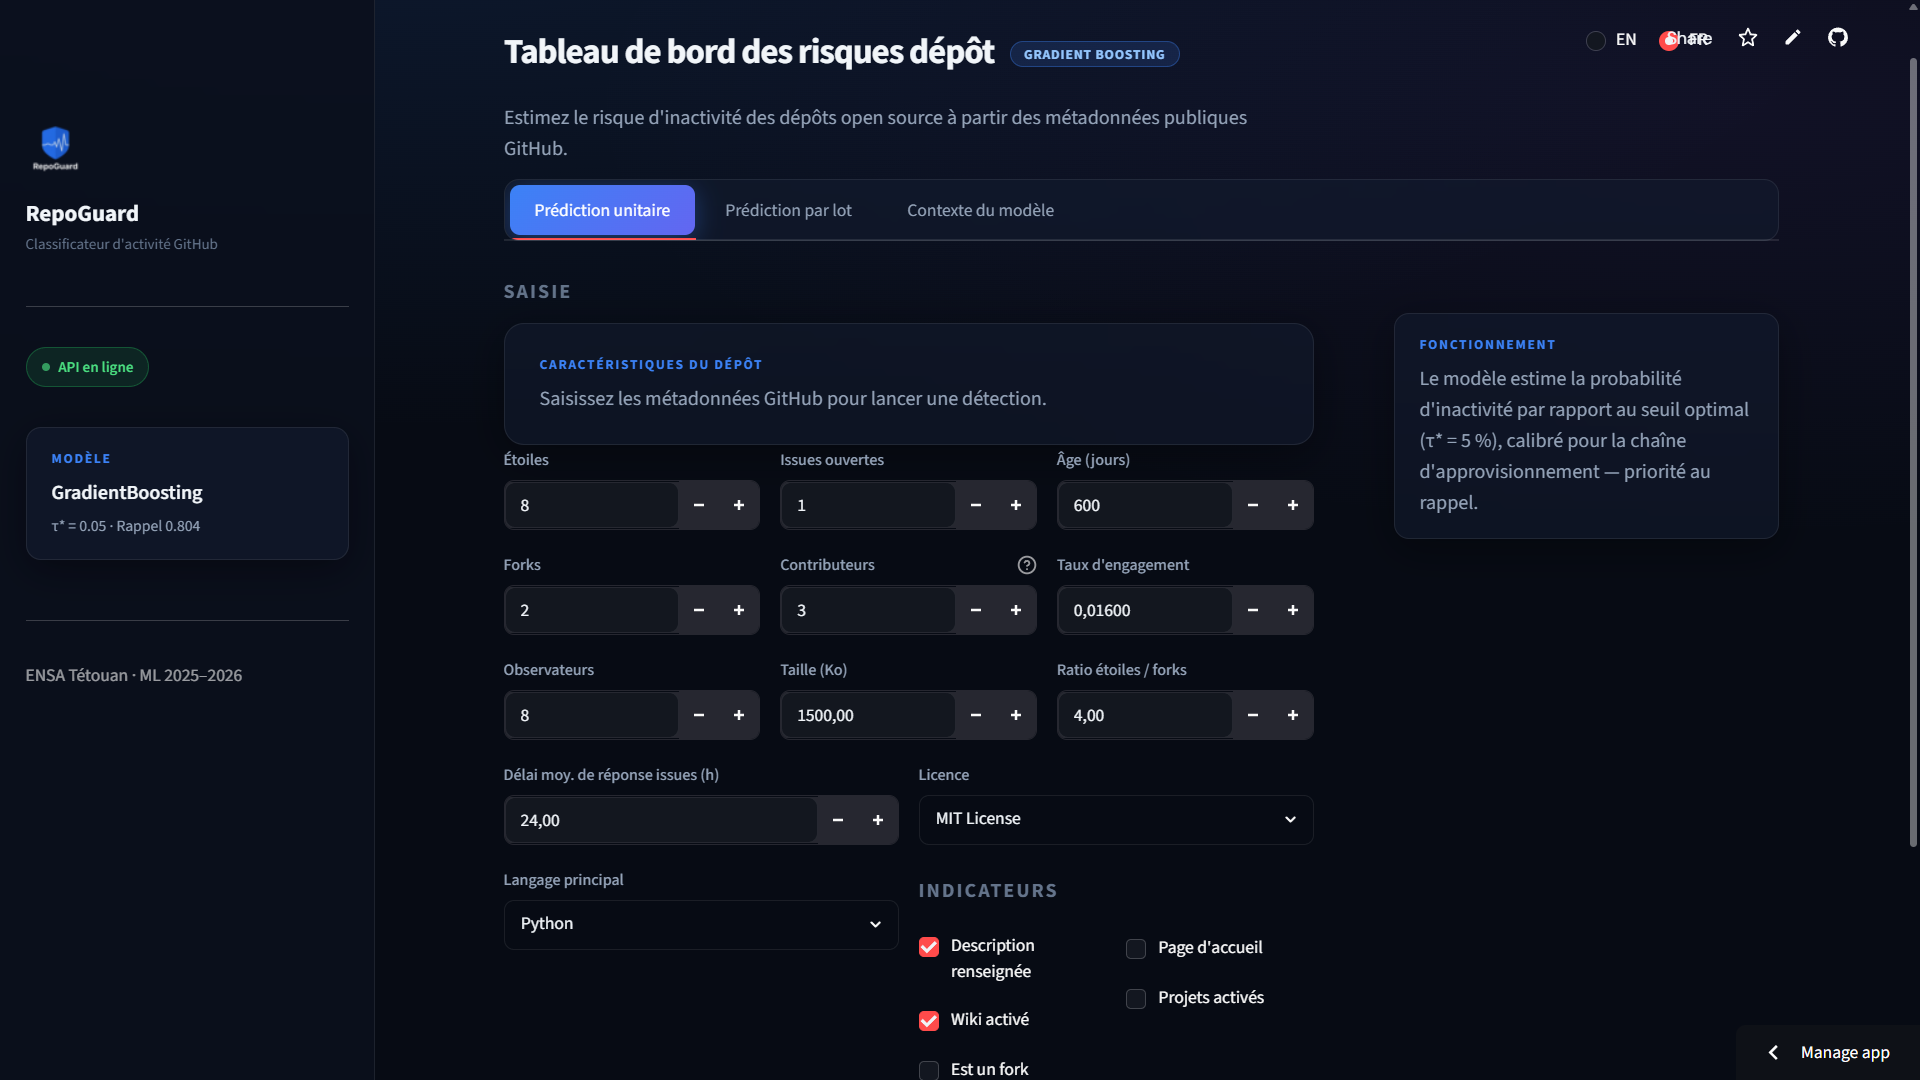
\includegraphics[width=0.92\textwidth]{screenshots/tab1_single}
  \caption{Interface Streamlit --- Onglet 1 : Prédiction Unitaire}
  \label{fig:tab_single}
\end{figure}

\begin{figure}[H]
  \centering
  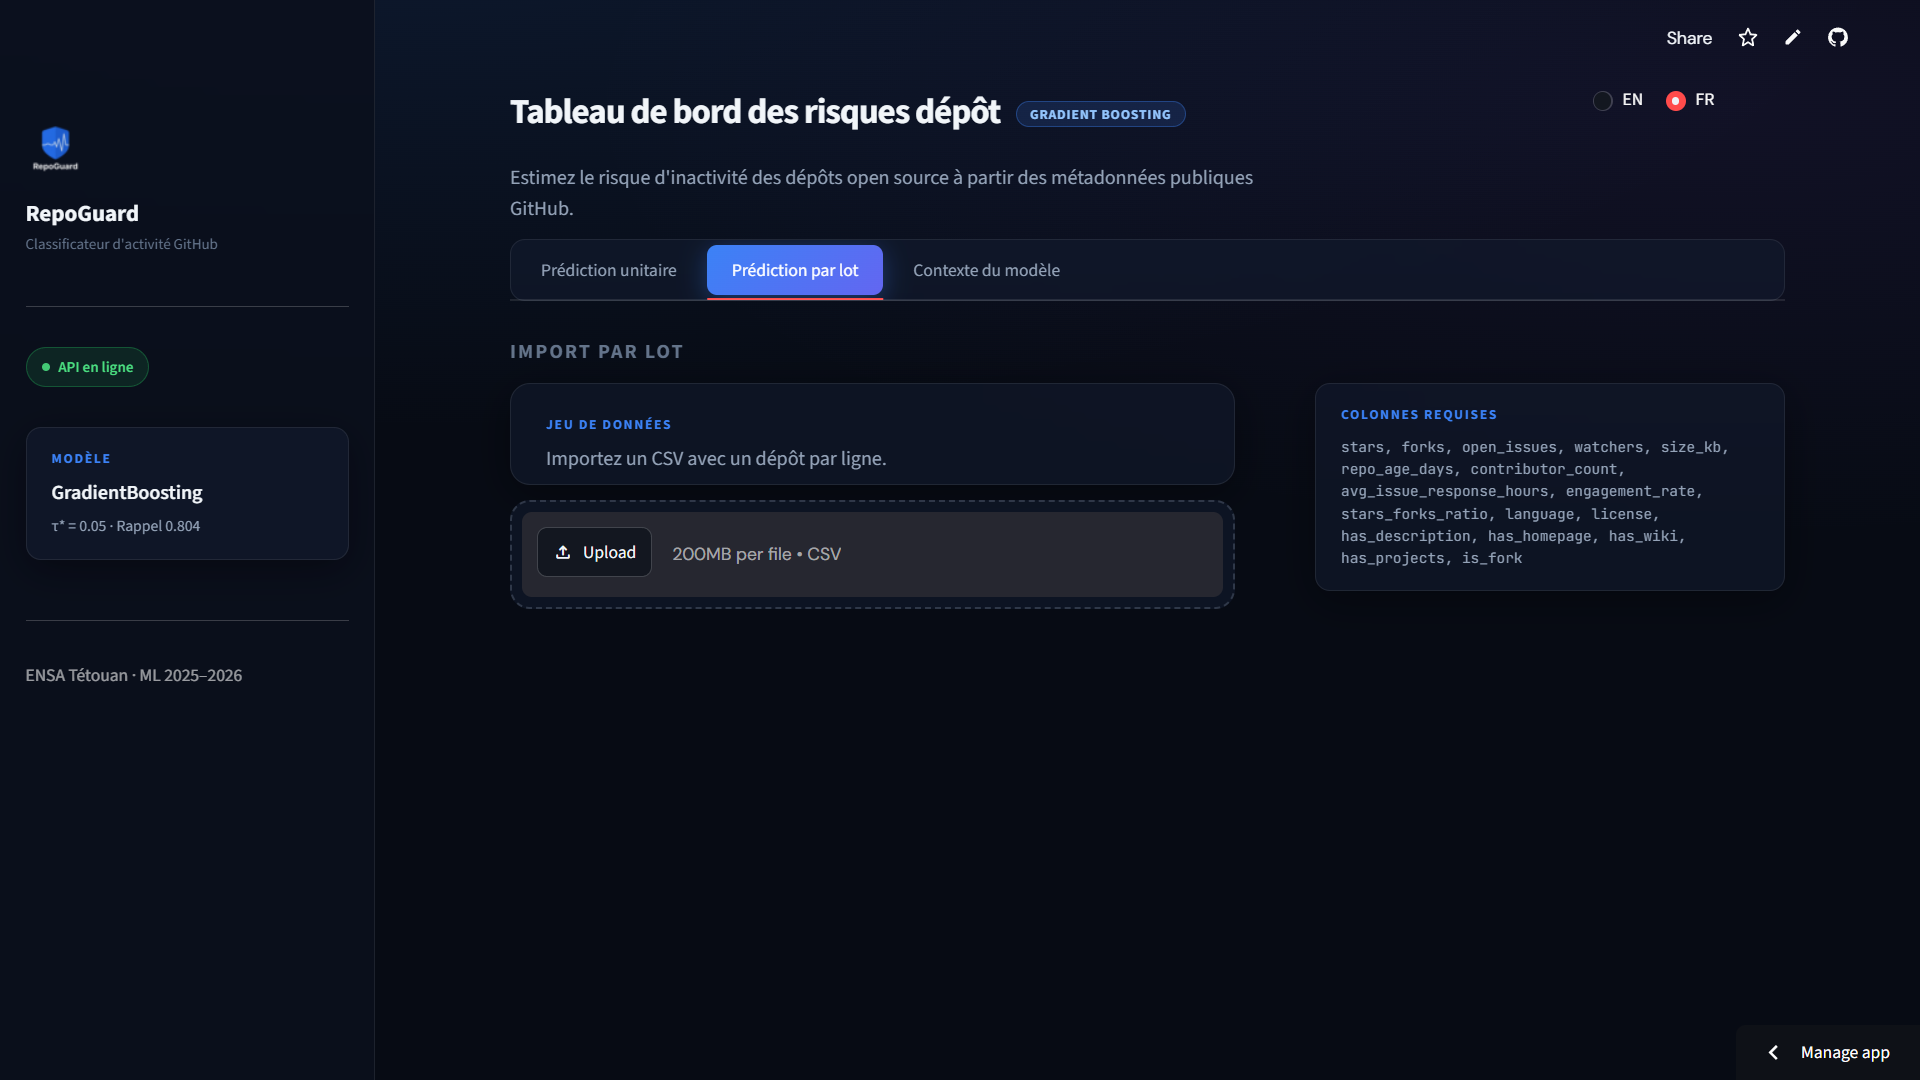
\includegraphics[width=0.92\textwidth]{screenshots/tab2_batch}
  \caption{Interface Streamlit --- Onglet 2 : Prédiction par Lot}
  \label{fig:tab_batch}
\end{figure}

\begin{figure}[H]
  \centering
  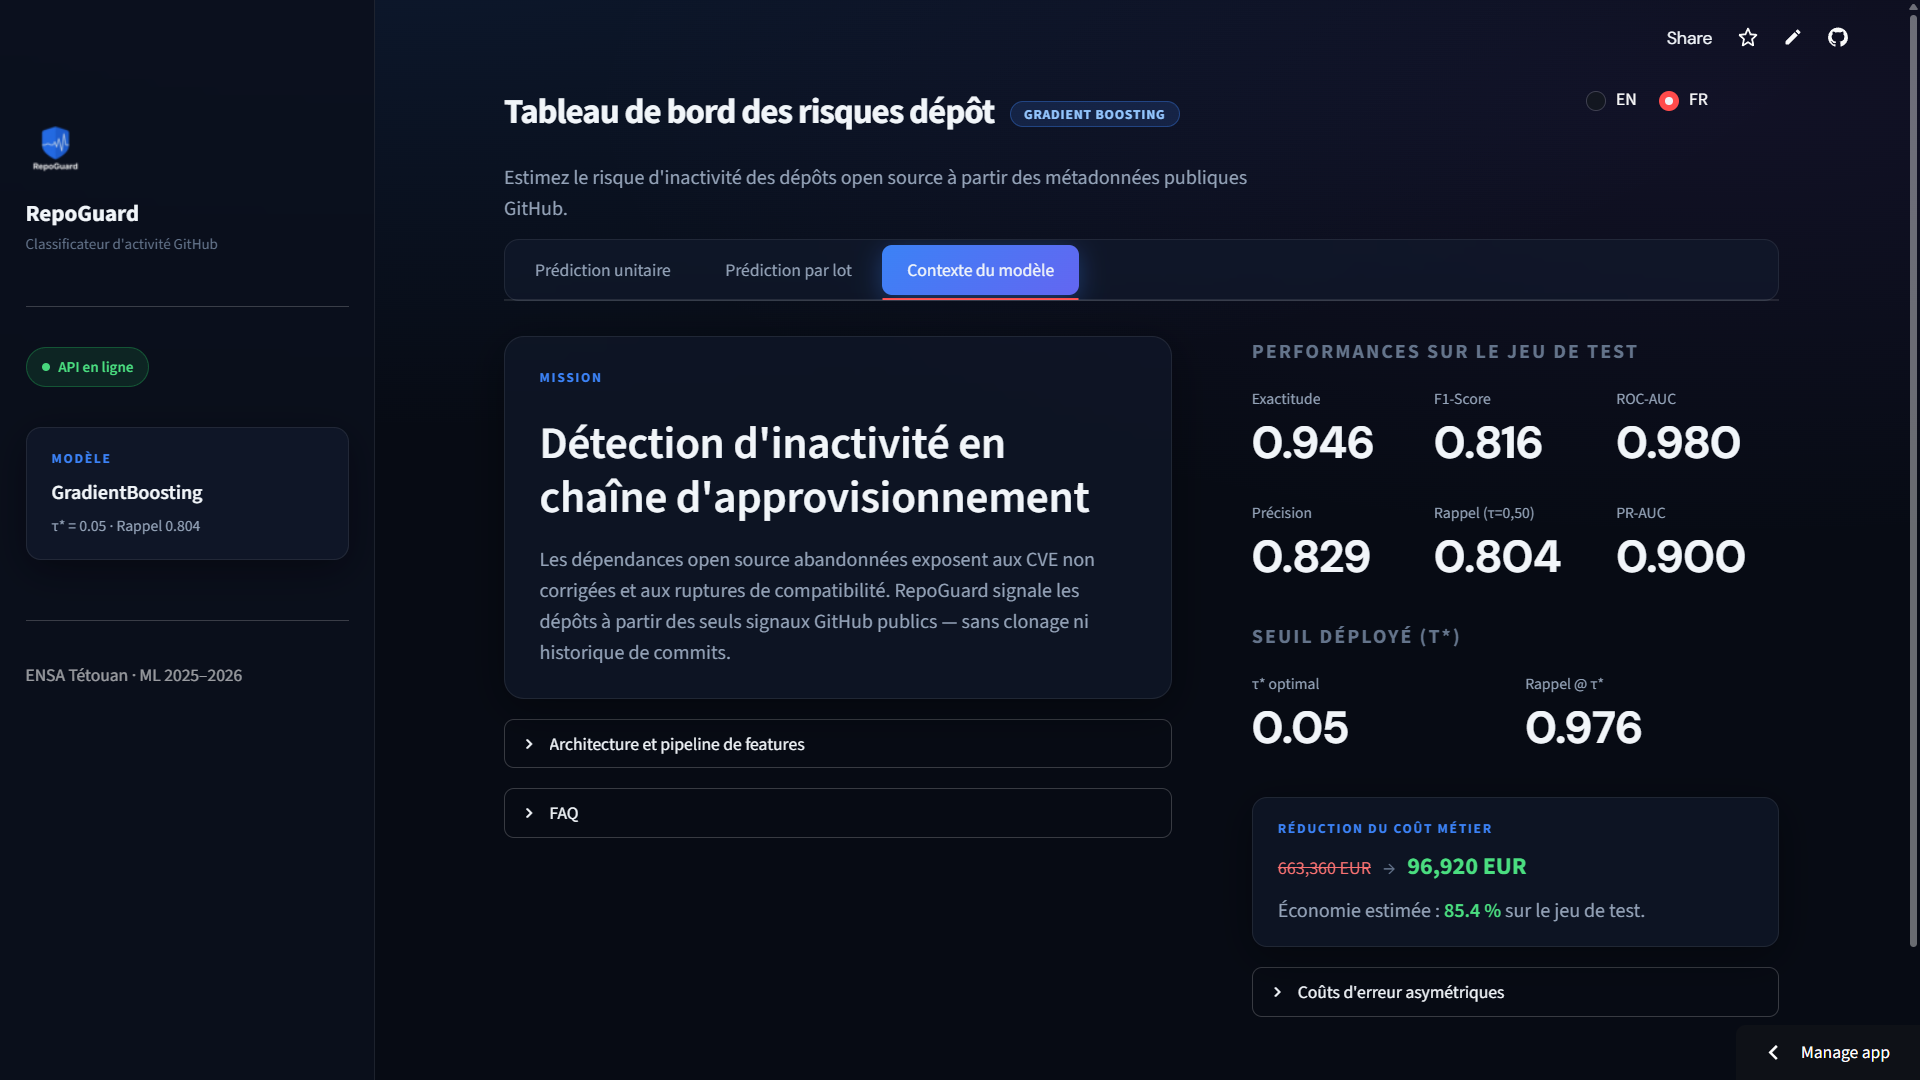
\includegraphics[width=0.92\textwidth]{screenshots/tab3_info}
  \caption{Interface Streamlit --- Onglet 3 : Informations Modèle \& Contexte Métier}
  \label{fig:tab_info}
\end{figure}

\subsection{Conteneurisation Docker}

\subsubsection{Structure des fichiers Docker}

\begin{itemize}[noitemsep]
  \item \textbf{Dockerfile} : image \texttt{python:3.11-slim} ; installation de
    \texttt{requirements.txt} avant la copie du code (optimisation du cache de couches).
  \item \textbf{.dockerignore} : exclut \texttt{data/}, \texttt{notebooks/}, \texttt{.git},
    \texttt{venv}, \texttt{\_\_pycache\_\_}.
  \item \textbf{docker-compose.yml} : orchestre les services \texttt{api} et \texttt{ui} sur
    un réseau virtuel partagé avec healthcheck configuré.
\end{itemize}

\subsubsection{Démarrage de l'application}

\begin{lstlisting}[language=bash, caption={Démarrage avec Docker Compose}]
docker-compose up --build
# Interface UI   : http://localhost:8500
# API Swagger    : http://localhost:8000/docs
# Health check   : http://localhost:8000/health
\end{lstlisting}

\subsection{Tests unitaires}

Des tests Pytest (\texttt{tests/test\_api.py}) couvrent :
\begin{itemize}[noitemsep]
  \item Validation des schémas Pydantic (types et contraintes de plage).
  \item Logique de Feature Engineering (\texttt{activity\_score}, \texttt{issues\_per\_contributor},
    \texttt{age\_category}).
  \item Calcul des niveaux de confiance (\texttt{get\_confidence\_level}).
\end{itemize}

\begin{lstlisting}[language=bash, caption={Exécution des tests unitaires}]
python -m pytest tests/ -v
\end{lstlisting}

\subsection{Variables d'environnement}

\begin{table}[H]
  \centering
  \caption{Variables d'environnement configurables}
  \label{tab:env}
  \begin{tabularx}{\linewidth}{llL}
    \toprule
    \textbf{Variable} & \textbf{Valeur par défaut} & \textbf{Description} \\
    \midrule
    \texttt{MODEL\_PATH} & \texttt{models/final\_model.joblib} & Chemin vers le pipeline sérialisé \\
    \texttt{METADATA\_PATH} & \texttt{models/final\_model\_metadata.json} & Chemin vers les métadonnées \\
    \texttt{API\_URL} & \texttt{http://localhost:8000} & URL de l'API (côté Streamlit) \\
    \bottomrule
  \end{tabularx}
\end{table}

% ============================================================
%  SECTION 6 (suite) — DÉPLOIEMENT EN PRODUCTION (CLOUD)
% ============================================================
\subsection{Déploiement en production (Cloud)}

L'application a été déployée en production sur deux plateformes cloud complémentaires,
accessibles publiquement sans installation locale.

\begin{table}[H]
  \centering
  \caption{Services déployés en production}
  \label{tab:deploy_cloud}
  \begin{tabularx}{\linewidth}{llL}
    \toprule
    \textbf{Service} & \textbf{Plateforme} & \textbf{URL de production} \\
    \midrule
    API REST (FastAPI + Uvicorn) & Railway &
      \url{https://github-repo-activity-classifier-production.up.railway.app} \\
    Interface utilisateur (Streamlit) & Streamlit Cloud &
      \url{https://app-repo-activity-classifier.streamlit.app} \\
    \bottomrule
  \end{tabularx}
\end{table}

\begin{keybox}[Accès rapide aux services déployés]
\begin{itemize}[noitemsep]
  \item \textbf{Interface utilisateur (Streamlit Cloud) :}\\
        \url{https://app-repo-activity-classifier.streamlit.app}
  \item \textbf{Documentation interactive de l'API (Swagger UI) :}\\
        \url{https://github-repo-activity-classifier-production.up.railway.app/docs}
  \item \textbf{Health check de l'API :}\\
        \url{https://github-repo-activity-classifier-production.up.railway.app/health}
  \item \textbf{Métadonnées du modèle :}\\
        \url{https://github-repo-activity-classifier-production.up.railway.app/model/info}
\end{itemize}
\end{keybox}

\subsubsection{API --- Railway}

Railway est une plateforme \textit{Platform-as-a-Service} (PaaS) qui déploie directement à
partir du dépôt Git. Le service API utilise l'image Docker définie dans le \texttt{Dockerfile}
du projet ; Railway détecte automatiquement le port exposé (\texttt{8000}) et attribue un
sous-domaine HTTPS sécurisé.

\begin{itemize}[noitemsep]
  \item \textbf{Déclencheur de déploiement} : push sur la branche \texttt{main} du dépôt GitHub.
  \item \textbf{Runtime} : conteneur Docker (\texttt{python:3.11-slim}) avec les modèles
    sérialisés (\texttt{models/}) embarqués dans l'image.
  \item \textbf{Variables d'environnement} : \texttt{MODEL\_PATH} et \texttt{METADATA\_PATH}
    configurés dans le tableau de bord Railway.
  \item \textbf{HTTPS} : certificat TLS automatiquement provisionné par Railway.
\end{itemize}

\subsubsection{Interface utilisateur --- Streamlit Cloud}

Streamlit Cloud héberge directement les applications Streamlit depuis un dépôt GitHub public.
L'interface est déployée à partir du fichier \texttt{app/ui.py}, avec la variable d'environnement
\texttt{API\_URL} pointant vers l'URL Railway en production.

\begin{itemize}[noitemsep]
  \item \textbf{Configuration} : fichier \texttt{.streamlit/secrets.toml} pour injecter
    \texttt{API\_URL=https://github-repo-activity-classifier-production.up.railway.app}.
  \item \textbf{Redéploiement automatique} : à chaque push sur \texttt{main}, Streamlit Cloud
    recharge l'application sans interruption.
  \item \textbf{Accès public} : aucune authentification requise, accessible depuis n'importe quel
    navigateur web.
\end{itemize}

% ============================================================
%  SECTION 7 — CONCLUSION, LIMITES ET PERSPECTIVES
% ============================================================
\newpage
\section{Conclusion, limites et perspectives}

\subsection{Bilan du projet}

Ce projet a couvert l'intégralité du cycle de vie CRISP-DM, de la collecte de données jusqu'au
déploiement en production :

\begin{enumerate}
  \item \textbf{Cadrage et collecte} : jeu de données original de 15\,000 dépôts GitHub, stratégie
    d'échantillonnage validée par la littérature académique, ratio de déséquilibre cohérent avec les
    mesures de Avelino et al.~(2019).
  \item \textbf{EDA et preprocessing} : analyse exploratoire complète, Feature Engineering de
    3 nouvelles variables justifiées métier, pipeline reproductible sérialisé.
  \item \textbf{Modélisation et tuning} : 12 configurations comparées rigoureusement. Gradient
    Boosting + class\_weight sélectionné. Tuning par GridSearchCV : F1 validation amélioré à 0,831.
  \item \textbf{Évaluation} : \textbf{tous les objectifs ML sont atteints dès le seuil par défaut}.
    L'optimisation du seuil à 0,05 réduit le coût métier estimé de \textbf{85,4\,\%}.
  \item \textbf{Déploiement} : API REST FastAPI + interface Streamlit + Docker Compose,
    avec tests unitaires et documentation Swagger auto-générée. L'application est déployée
    en production sur \textbf{Railway} (API) et \textbf{Streamlit Cloud} (interface), et
    accessible publiquement à \url{https://app-repo-activity-classifier.streamlit.app}.
\end{enumerate}

\subsection{Limites identifiées}

\begin{enumerate}[label=\textbf{L\arabic*.}]
  \item \textbf{Seuil très agressif (0,05)} : précision de 0,54 au seuil optimal --- environ la
    moitié des alertes sont des faux positifs. Ce choix délibéré peut générer une fatigue d'alerte
    à grande échelle.
  \item \textbf{\texttt{contributor\_count} plafonné à 100} : les grands projets communautaires
    ont une valeur tronquée, sous-estimant potentiellement leur robustesse.
  \item \textbf{Délai de réponse aux issues estimé sur 20 issues} : peut masquer des évolutions
    récentes de l'activité.
  \item \textbf{Absence de fréquence de commits} : non disponible directement via les endpoints
    utilisés, malgré sa haute pertinence prédictive.
  \item \textbf{Snapshot temporel} : le jeu de données est une photo à une date précise
    (2026-05-15) ; le modèle ne capture pas les dynamiques temporelles intra-projet.
  \item \textbf{Couverture linguistique limitée} : 10 langages ; les projets dans des langages
    de niche sont regroupés en \texttt{Other}.
\end{enumerate}

\subsection{Perspectives d'amélioration}

\begin{enumerate}[label=\textbf{P\arabic*.}]
  \item \textbf{Données de commits} : exploiter \texttt{/stats/commit\_activity} pour la
    fréquence hebdomadaire des commits.
  \item \textbf{Explicabilité SHAP} : intégrer \texttt{shap.TreeExplainer} pour des
    explications individualisées dans l'interface.
  \item \textbf{Modèle séquentiel / temporel} : snapshots mensuels + modèle de survie ou
    LSTM pour une prédiction à horizon variable.
  \item \textbf{Monitoring du drift} : Evidently AI pour détecter les dérives de distribution
    en production.
  \item \textbf{Corrélation avec les registres de paquets} : croiser avec le nombre de
    téléchargements npm/PyPI pour un signal de dépendance réelle plus direct.
  \item \textbf{Seuils personnalisés par profil d'utilisation} : seuils différenciés selon
    le contexte (équipe sécurité vs.\ développeur individuel) pour réduire la fatigue d'alerte.
\end{enumerate}

% ============================================================
%  RÉFÉRENCES
% ============================================================
\newpage
\bibliographystyle{plainnat}
\begin{thebibliography}{5}

\bibitem{avelino2019}
Avelino, G., Constantinou, E., Mens, T., \& Serebrenik, A. (2019).
\textit{A Novel Approach for Estimating Truck Factors}.
In \textit{Proceedings of the 16th International Conference on Mining Software
Repositories (MSR 2019)}.
\url{https://doi.org/10.1109/MSR.2019.00059}

\bibitem{sonatype2023}
Sonatype. (2023).
\textit{State of the Software Supply Chain 2023}.
\url{https://www.sonatype.com/state-of-the-software-supply-chain}

\bibitem{snyk2023}
Snyk. (2023).
\textit{State of Open Source Security 2023}.
\url{https://snyk.io}

\bibitem{chawla2002}
Chawla, N. V., Bowyer, K. W., Hall, L. O., \& Kegelmeyer, W. P. (2002).
\textit{SMOTE: Synthetic Minority Over-sampling Technique}.
\textit{Journal of Artificial Intelligence Research}, 16, 321--357.
\url{https://doi.org/10.1613/jair.953}

\bibitem{fastapi}
Ramírez, S. (2019).
\textit{FastAPI --- framework for building APIs with Python}.
\url{https://fastapi.tiangolo.com}

\end{thebibliography}

% ============================================================
%  ANNEXES
% ============================================================
\newpage
\appendix
\section{Annexe A --- Extraits de code clés}

\subsection{Stratégie d'échantillonnage en deux passes}

\begin{lstlisting}[style=python, caption={Stratégie de collecte en deux passes (extrait de src/data\_collection.py)}, label=lst:collection]
CUTOFF_DATE = "2025-11-15"   # 180 jours avant la date de collecte

# Passe 1 : depots inactifs garantis
query_inactive = (
    f"stars:{star_range} language:{lang} "
    f"pushed:<{CUTOFF_DATE} size:>=1"
)
repos_inactive = search_repositories(query_inactive, max_results=per_cell)

# Passe 2 : depots actifs garantis
query_active = (
    f"stars:{star_range} language:{lang} "
    f"pushed:>{CUTOFF_DATE} size:>=1"
)
repos_active = search_repositories(query_active, max_results=per_cell)
\end{lstlisting}

\subsection{Feature Engineering côté API}

\begin{lstlisting}[style=python, caption={Feature engineering dans l'API (app/api.py)}, label=lst:fe_api]
def preprocess_single(item: RepoInput) -> pd.DataFrame:
    raw = {
        "stars": item.stars, "forks": item.forks,
        "open_issues": item.open_issues, ...
    }
    # Traitement de la valeur sentinelle -1.0
    if raw["avg_issue_response_hours"] == -1.0:
        raw["avg_issue_response_hours"] = np.nan

    # Feature Engineering (identique a l'entrainement)
    raw["activity_score"] = raw["stars"] + raw["forks"] + raw["watchers"]
    raw["issues_per_contributor"] = (
        raw["open_issues"] / (raw["contributor_count"] + 1)
    )
    raw["age_category"] = categorize_age(raw["repo_age_days"])
    return pd.DataFrame([raw])

def categorize_age(days: int) -> str:
    if days < 180:   return 'nouveau'
    elif days < 730: return 'jeune'
    elif days < 1825: return 'mature'
    else:            return 'ancien'
\end{lstlisting}

\subsection{Optimisation du seuil de décision}

\begin{lstlisting}[style=python, caption={Calcul du seuil optimal par minimisation du coût métier}, label=lst:threshold]
FN_COST = 10_000  # EUR
FP_COST = 60      # EUR

thresholds = np.arange(0.01, 0.90, 0.01)
costs = []
for tau in thresholds:
    y_pred = (y_proba >= tau).astype(int)
    tn, fp, fn, tp = confusion_matrix(y_test, y_pred).ravel()
    costs.append(FN_COST * fn + FP_COST * fp)

optimal_threshold = thresholds[np.argmin(costs)]
# Resultat : tau* = 0.05
# Cout optimal  : 96 920 EUR
# Cout defaut   : 663 360 EUR
# Reduction     : -85.4%
\end{lstlisting}

\section{Annexe B --- Métadonnées du modèle final}

\begin{lstlisting}[caption={Contenu de models/final\_model\_metadata.json}, label=lst:metadata, language={}]
{
  "pipeline_path": "models/final_model.joblib",
  "optimal_threshold": 0.05,
  "default_threshold": 0.5,
  "model_name": "GradientBoosting",
  "strategy": "class_weight",
  "best_params": {
    "classifier__max_depth": "3",
    "classifier__learning_rate": "0.1",
    "classifier__n_estimators": "300",
    "classifier__subsample": "1.0",
    "classifier__min_samples_leaf": "1"
  },
  "test_metrics_default": {
    "recall": 0.8042, "precision": 0.8287, "f1": 0.8163,
    "roc_auc": 0.9797, "pr_auc": 0.8999, "accuracy": 0.9458
  },
  "test_metrics_optimal": {
    "recall": 0.9763, "precision": 0.5385,
    "f1": 0.6941, "total_cost": 96920.0
  },
  "cost_matrix": {
    "FN_cost": 10000, "FP_cost": 60,
    "cost_default": 663360.0, "cost_optimal": 96920.0
  }
}
\end{lstlisting}

\section{Annexe C --- Arborescence du projet}

\begin{lstlisting}[language={}, caption={Structure du dépôt Git}]
github-repo-activity-classifier/
|-- app/
|   |-- api.py             # API REST FastAPI
|   `-- ui.py              # Interface Streamlit
|-- data/
|   |-- processed/         # train.csv, validation.csv, test.csv
|   `-- dataset.csv        # Dataset complet (15 000 lignes)
|-- docs/
|   |-- screenshots/
|   |   |-- tab1_single.png
|   |   |-- tab2_batch.png
|   |   `-- tab3_info.png
|   |-- ensate_logo.png    # Logo ENSA Tetouan
|   `-- main.tex           # Rapport LaTeX
|-- models/
|   |-- final_model.joblib
|   |-- final_model_metadata.json
|   |-- preprocessor.joblib
|   `-- tuning_metadata.json
|-- notebooks/
|   |-- 01_discovery.ipynb
|   |-- 02_eda.ipynb
|   |-- 03_preprocessing.ipynb
|   |-- 04_modeling.ipynb
|   |-- 05_tuning.ipynb
|   `-- 06_evaluation.ipynb
|-- src/
|   `-- data_collection.py
|-- tests/
|   `-- test_api.py
|-- Dockerfile
|-- docker-compose.yml
|-- requirements.txt
`-- README.md
\end{lstlisting}

\end{document}

